\section{Evaluation}\label{sec:evaluation}

%\paragraph{Application to the ETCS specification}

\begin{figure}
\centering
\resizebox{\linewidth}{!}{
\begin{tikzpicture}
\node[initialstate] (initial) {};
\node[smstate,left=0.2cm of initial] (normal) {Normal\\/entry\\tco=0;\\sb=0;\\eb=0;};
\node[smstate,left=1.5cm of normal] (indication) {Indication};
\node[smstate,left= 1cm of indication] (overspeed) {Overspeed};
\node[smstate,above=2cm of overspeed] (warning) {Warning\\/entry\\tco=1;};
\node[smstate,above=2cm of indication] (sb) {SB\\/entry\\sb=1;};
\node[smstate] at(sb-|normal) (eb) {EB\\/entry\\eb=1;};

\draw[trans] (initial) -- (normal);
\draw[trans] (normal) --node[below] {$[t_3]$} (indication);
\draw[trans] (indication) -- node[below] {$[t_4]$}(overspeed);
\draw[trans] (overspeed) -- node[left] {$[t_7]$}(warning);
\draw[trans] (warning) -- node[above] {$[t_{10}]$}(sb);
\draw[trans] (sb) -- node[above] {$[t_{13}]$}(eb);
\draw[trans] (eb) -- node[right] {$[r_0]$}(normal);

\draw[trans] (indication) -- node[above,pos=1.0] {$[r_{1}||r_2]$} ($(indication)!0.5!(normal) + (0,0.5cm)$) -- (normal);
\draw[trans] (overspeed) -- node[above,pos=1.0] {$[r_3]$} ($(overspeed)!0.5!(indication) + (0,0.5cm)$) -- (indication);

\draw[trans] (warning) -- node[above right] {$[r_3]$}(indication);
\draw[trans] (sb) -- node[right] {$[r_3]$}(indication);
\end{tikzpicture}
}
\caption{State Machine of the TSM}
\label{fig:statemachine}
\end{figure}

\begin{figure*}[h]
\centering
\begin{tikzpicture}
\node[constraint] (c1) {$\lbrace t_{13} = v > (v_m + DV_\text{ebi}) \vee D_f > D_e\rbrace$};
\node[constraint, below=of c1] (c2) {$DV_\text{ebi} = 
   \left\{
   \begin{aligned}
   &7.5 & \IF v_m\leq 110\\
   &0.075 v_m-0.75 &\IF 110\le v_m \leq 210\\
   &15 & \IF 210 \leq v_m
   \end{aligned}
   \right. $
   };
\node[constraint, right=2 of c1] (c3) {$\lbrace D_\text{EBI} = D_e - T_\text{be} v \rbrace$};
\node[constraint, below=of c3] (c4) {$\lbrace D_\text{EBD} = D_t - s\rbrace $};


\node[parameter, left=1.5cm of c1, left= of c1] (df) {$D_\text{front}$};

\node[parameter, right=of c4] (dt) {$D_\text{target}$};
\node[parameter, below=0.5cm of dt] (s) {$s$};

\node[parameter, below=0.5cm of df] (vm) {$v_\text{mrsp}$};
\node[parameter, right=of c3] (tb) {$T_\text{be}$};
\node[parameter, above=0.4cm of tb] (ve) {$v_\text{est}$};

\draw[binding] (df) -- node[above] {$D_f$} (c1);
\draw[binding] (ve) -| node[near end, left] {$v$} (c1.50);
\draw[binding] (ve) -| node[near end, right] {$v$}(c3);
\draw[binding] (vm) -| node[near end, left] {$v_m$}(c1.200);
\draw[binding] (vm) -| node[near end, right] {$v_m$}(c2.150);
\draw[binding] (dt) -- node[above] {$D_t$} (c4);
\draw[binding] (s) -| node[near end, left] {$s$} (c4);
\draw[binding] (tb) -- node[above] {$T_\text{be}$}(c3);

\draw[double binding] (c1) -- node[right] {$DV_\text{ebi}$} ($(c2)!0.6!(c1)$) -| node [near end, right] {$DV_\text{ebi}$} (c2.21);
\draw[double binding] (c1) -- node[near start, above] {$D_\text{e}$} node [near end, below] {$D_\text{EBI} $}  (c3);
\draw[double binding] (c3) -- node[near start, right] {$D_\text{e}$} node [near end, left] {$D_\text{EBD}$} (c4);



\end{tikzpicture}
\caption{Parametric Diagram of the TSM}
\label{fig:parametric}
\end{figure*}



The approach described in the previous sections has been applied to the TSM function of the ETCS specification~\cite{ETCSSRS-Principles}. The specification describes the behavior in means of a transition table with the corresponding conditions for each transition. Such a specification can easily be modeled in terms of state machines and parametric diagrams: 
For every condition defined in the specification a Boolean variable $t_3,\ldots,t_{13},$ $r_0,\ldots,r_3$ was introduced, named according to the definitions  in~\cite{ETCSSRS-Principles}. The state machine can easily be deduced from the transition table using the introduced Boolean variables. The corresponding state machine of the TSM function is shown in Figure~\ref{fig:statemachine}. The concrete conditions are described and the introduced Boolean variables are bound by means of parametric diagrams. An excerpt of the parametric diagram of the TSM function is given in Figure~\ref{fig:parametric}. 

As a result, specifying the constraint blocks and creating the parametric diagram, as well as the state machine, was straightforward, where only the mathematical equations given in \cite{ETCSSRS-Principles} had to be translated to
constraint blocks and some notations had to be slightly modified to be parsed by our tools. Thus, the 
modeling effort for this example was very low and we assume that the modelling effort should scale very well
if other sub functions of this specification were modeled with the proposed approach.  

\paragraph{Model description}
In the TSM function state changes occur as soon as trigger conditions are fulfilled.
Under certain trigger conditions ($t_3$,$t_4$, \ldots) the system changes
its state machine state corresponding to different levels of intervention.
$t_3$ is a boolean expression that evaluates to true, if the current velocity
$V_\text{est}$ and the current train front position $D_\text{front}$ exceed the
line indicated by $D_I$ in Figure~\ref{fig:braking-curves}. Similarly,
$t_4,t_7,t_{10}$ and $t_{13}$ return true if and only if the train
exceeds $D_\text{P},D_\text{W},D_\text{SBI}$ or $D_\text{EBI}$ respectively.
When a new state machine state is entered, the \emph{entry}-actions write to the output
variables $\text{tco},\text{sb}$ and $\text{eb}$. These variables indicate the
activation of the traction cut-off, the service brake and the emergency brake.
The revocation conditions $r_0,\ldots,r_3$ describe the conditions
necessary for the intervention states to be revoked.

%figure for one column
%figure* for two column figures
\begin{figure}[b]
\centering
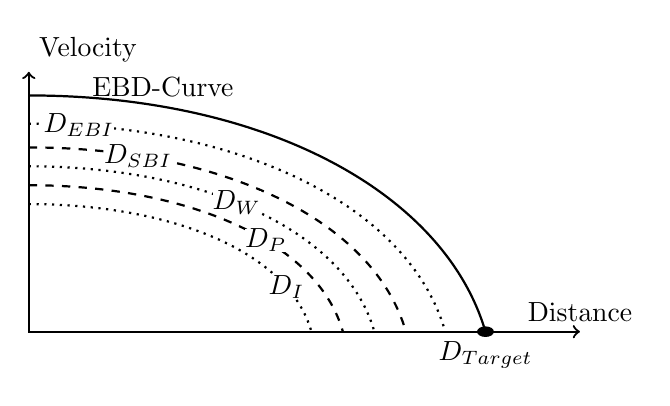
\begin{tikzpicture}[yscale=0.6]
% \draw[thick,red,xstep=1,ystep=1] (0,0) grid (8,6);
% \draw[very thin,red,xstep=0.1,ystep=0.1] (0,0) grid (8,6);
\draw[<->,thick] (0,5.5) node[above right] {Velocity} -- (0,0) -- (7,0) node[above] {Distance};
\node[below] (ebdfoot) at (5.8,0) {$D_\text{Target}$};
\draw[fill] (5.8,0) circle [radius=0.1];
\draw[thick] (0,5) to [out=0,in=100]  node[pos=0.2,above]{EBD-Curve} (5.8,0);
\node[below right] (ebifoot) at (5.2,0) {};
\draw[thick,dotted] (0,4.4) to [out=0,in=100] node[fill=white,inner sep=0,pos=0.08]{$D_\text{EBI}$} (ebifoot);
\node[below right] (sbifoot) at (4.7,0) {};
\draw[thick,dashed] (0,3.9) to [out=0,in=100] node[fill=white,inner sep=0,pos=0.2]{$D_\text{SBI}$} (sbifoot);
\node[below right] (wfoot) at (4.3,0) {};
\draw[thick,dotted] (0,3.5) to [out=0,in=100] node[fill=white,inner sep=0,pos=0.45]{$D_\text{W}$} (wfoot);
\node[below right] (pfoot) at (3.9,0) {};
\draw[thick,dashed] (0,3.1) to [out=0,in=100] node[fill=white,inner sep=0,pos=0.6]{$D_\text{P}$} (pfoot);
\node[below right] (ifoot) at (3.5,0) {};
\draw[thick,dotted] (0,2.7) to [out=0,in=100] node[fill=white,inner sep=0,pos=0.8]{$D_\text{I}$} (ifoot);
\end{tikzpicture}
\caption{Braking Curves of the TSM}
\label{fig:braking-curves}
\end{figure}   

The \emph{state invariants} of our test model are described by means of a parametric diagram and as an example in Figure~\ref{fig:parametric} the definition of trigger condition $t_{13}$ is shown. For convenience the definition of the other triggering conditions is omitted. 


All these triggering conditions depend on the train velocity and track relative
distance (position). The conditions can be calculated from the EBD
curve, compare Figure~\ref{fig:braking-curves}.
The EBD curve (emergency brake deceleration) maps the track relative distance to a
velocity, assuming a negative acceleration $A_\text{safe}$, such that zero speed is reached
at the target position ($D_\text{Target}$). The curve can be calculated by calculation of the 
braking distance $s$ as shown in Figure~\ref{fig:brakingdistance}.
The value of $A_\text{safe}$\footnote{For convenience we used a fixed value for
$A_\text{safe}$. According to the ETCS specification
\cite{ETCSSRS-Principles} up to seven values can be defined as a step function
dependent on the train speed.} is a conservative approximation that describes
the least deceleration that the emergency brakes of the train achieve when
fully activated.
Because the full activation of the emergency brakes needs some time, the curve
$D_\text{EBI}$ is shifted by a fixed time delay.
If the current distance-velocity-pair describing the train speed and position is
right or above this line, the emergency brakes are triggered.
In a similar way the other triggering conditions are defined by shifting the EBD
cure by fixed time delays.
   

The \emph{temporal evolution} of our test model is described by the parametric
diagram shown in Figure~\ref{fig:temporal-evolution}. The constraints in this diagram
restrict the time-continuous evolution of the trains front position and the velocity.
Therefore the acceleration $a$ of the train is restricted to values in the range $[-10,2]$. 
If the emergency brakes are activated (the train is in the state machine
state EB), the deceleration must be higher than prescribed by $A_\text{safe}$.  
As described in section~\ref{sec:concretization}, the discretized versions of
the constraints were used.

In total, our test model used for this evaluation contains 52 constraint properties,
including those shown in Figure~\ref{fig:brakingdistance},\ref{fig:temporal-evolution} and \ref{fig:parametric}.

\paragraph{Test case generation}

Table~\ref{tab:testgen} gives a summary of our test case generation. The test
case generation was performed on a system with 24 CPU cores running at 2.8 GHz
with 16 GB RAM. In the first step of our test case generation 50 abstract test
cases were calculated, which took less than a second. 
Then it took three and a half hours to generate the concrete test
cases from the 50 abstract test cases. The main reason, that this
computationally expensive task, is still applicable in acceptable time, is that
SMT instances for every test case can be solved in parallel. The test case
generation was run in parallel and on average 16.7 of the 24 CPUs were
utilized.

Given that the results from this TSM model can be generalized to hybrid systems
of comparable complexity, the runtime is acceptable. Yet, the
results indicate, that the utilization of a different computational backend,
e.g. analytical or numerical solvers, should be considered.

For every abstract test case a concrete
solution was calculated. Thus, our model abstraction seems appropriate. This might not always
be the case. If the test case generation of abstract test cases yields a low
percentage of solvable concrete test cases, this might be an indicator for
inappropriate abstraction or too restrictive constraints.


\begin{table}[h]
\centering
\begin{tabular}{|p{0.6\linewidth}|p{0.3\linewidth}|}
\hline
number of test cases generated & 50 \\
\hline
avg. test case length (test steps) & $2.84$ \\
 \hline
time for abstract test case generation & $0.8s$ \\
 \hline
time for calculation of concrete test cases & $3.5h$ \\
 \hline
 memory for test case generation & 8.4 GB\\
 \hline 
\end{tabular}
\caption{Results of the Test Case Generation for the TSM Model}
\label{tab:testgen}
\end{table}